\chapter{Từ các mode động lượng đến các trường lượng tử cục bộ}

Trường lượng tử là gì, và nó liên hệ với các hạt như thế nào? Công cụ toán học cơ bản là dao động tử điều hòa. Một trường chứa nhiều mode dao động khả dĩ, và việc lượng tử hóa trường tương đương với việc ghép một dao động tử điều hòa lượng tử cho mỗi mode. Cách xây dựng này dễ thấy nhất nếu trước tiên xét một không gian tuần hoàn hữu hạn, nơi các mode được phép tạo thành một danh sách rời rạc.

\section{Không gian tuần hoàn và các số sóng được phép}

Lấy một tọa độ không gian \(x\) và đồng nhất các điểm cách nhau một khoảng \(L\). Có thể hình dung không gian này như một đường tròn có chu vi \(L\). Đây là một thủ pháp thể tích hữu hạn hữu ích. Trên một khoảng hữu hạn có các đầu mút, một sóng truyền sẽ phản xạ ở các đầu. Trên một khoảng tuần hoàn, nó có thể tiếp tục theo một trong hai hướng mà không phản xạ. Đối xứng tịnh tiến, và vì thế là bảo toàn động lượng, được giữ lại trong khi những phức tạp của thể tích vô hạn được tạm thời loại bỏ.

Một sóng phẳng có dạng
\begin{equation}
e^{ikx}.
\end{equation}
Sau một vòng đi quanh đường tròn, nó phải trở về giá trị ban đầu. Vì sóng bằng \(1\) tại \(x=0\), tính tuần hoàn đòi hỏi
\begin{equation}
e^{ikL}=1.
\end{equation}
Vì sao một bội nguyên của \(2\pi\) lại thỏa mãn điều kiện này? Công thức Euler cho
\begin{align}
e^{i2\pi n}
&=\cos(2\pi n)+i\sin(2\pi n)\\
&=1,
\qquad n\in\mathbb Z.
\end{align}
Cosin bằng \(1\) và sin bằng \(0\) sau bất kỳ số nguyên chu kỳ nào. Do đó,
\begin{equation}
kL=2\pi n,
\qquad
k=\frac{2\pi n}{L},
\qquad n\in\mathbb Z.
\end{equation}
Đại lượng \(k\) là số sóng. Số nguyên \(n\) gắn nhãn một số sóng được phép; nó chưa dùng để đếm hạt.

Cùng điều kiện ấy cũng có thể được biểu diễn theo bước sóng. Bước sóng là khoảng cách mà trên đó pha tăng thêm một chu kỳ trọn vẹn, do đó
\begin{equation}
k\lambda=2\pi,
\qquad
k=\frac{2\pi}{\lambda}.
\end{equation}
Bước sóng dài thì có số sóng nhỏ, còn bước sóng ngắn thì có số sóng lớn. Điều kiện tuần hoàn nói rằng có một số nguyên bước sóng vừa khít quanh đường tròn.

Đối với một sóng cơ học lượng tử, động lượng là
\begin{equation}
p=\frac{h}{\lambda}
=\frac{2\pi\hbar}{\lambda}
=\hbar k.
\end{equation}
Do đó \(k\) và \(p\) chỉ khác nhau bởi hệ số \(\hbar\). \(k\) dương và âm mô tả các sóng chuyển động theo hai hướng đối nhau và các hạt có động lượng ngược hướng. Trong các đơn vị với \(\hbar=1\), người ta thường gọi \(k\) là động lượng mà không phân biệt thêm.

Với mỗi \(k\) được phép, có thể có một số lượng tử nào đó trong mode ấy. Điều này đưa vào một số nguyên thứ hai:
\begin{equation}
n(k)=\text{number of quanta with wave number }k.
\end{equation}
Nó được gọi là số chiếm đóng. Số nguyên trong \(k=2\pi n/L\) gắn nhãn mode; \(n(k)\) cho biết có bao nhiêu hạt chiếm mode đó. Phải cho các số chiếm đóng cho cả \(k\) âm lẫn dương.

\begin{classroomqa}
\lecturetimestamp{00:11:58}
\audiencequestion{Bản thân \(k\) có phải là một số nguyên không?}
\lecturerresponse{Không. Số sóng là một bội nguyên của \(2\pi/L\): \(k=2\pi n/L\). Số nguyên \(n\) trong công thức đó gắn nhãn động lượng được phép, và nó khác với số chiếm đóng \(n(k)\), là số đếm các lượng tử trong mode.}
\end{classroomqa}

\section{Các trạng thái số chiếm đóng và các toán tử mode}

Một trạng thái lượng tử là một vectơ, hay phần tử tuyến tính. Các vectơ trạng thái có thể được cộng với nhau và nhân với các số, còn các toán tử tác động lên chúng để tạo ra các vectơ trạng thái khác. Các đại lượng thực quan sát được được biểu diễn bởi các toán tử Hermite. Những sự kiện sơ đẳng này quan trọng ở đây vì cả trạng thái nhiều hạt lẫn trường đều sẽ được xây dựng từ các tổ hợp tuyến tính và các toán tử.

Đặt
\begin{equation}
k_j=\frac{2\pi j}{L},
\qquad j\in\mathbb Z.
\end{equation}
Một nhãn thuận tiện cho một trạng thái nhiều hạt là toàn bộ dãy số chiếm đóng. Dùng ký hiệu tắt \(n_j\equiv n(k_j)\) cho các phần tử đã hiển thị, viết
\begin{equation}
\big|\{n(k_j)\}\big\rangle
=
\big|\ldots,n_{-2},n_{-1},n_0,n_1,n_2,\ldots\big\rangle.
\end{equation}
Phần tử \(n(k_1)\) là số hạt trong mode động lượng dương thứ nhất, \(n(k_2)\) là số trong mode thứ hai, v.v. Dãy này kéo dài vô hạn về cả hai phía.

\begin{figure}[t]
\centering
\includegraphics[width=0.72\textwidth]{lecture_03_figure_02.png}
\caption{Số chiếm đóng \(n(k)\) cho một mode động lượng được phép.}
\lectureframe{00:15:04}
\end{figure}

Mỗi mode động lượng là một dao động điều hòa. Vì vậy nó có một toán tử nâng và một toán tử hạ. Ký hiệu ban đầu viết là \(a^{+}(k)\) và \(a^{-}(k)\) sẽ được viết là \(a^\dagger(k)\) và \(a(k)\). Tác dụng của chúng là
\begin{align}
a^\dagger(k)\big|\ldots,n(k),\ldots\big\rangle
&=
\sqrt{n(k)+1}\notag\\
&\quad{}\times
\big|\ldots,n(k)+1,\ldots\big\rangle,
\\
a(k)\big|\ldots,n(k),\ldots\big\rangle
&=
\sqrt{n(k)}\,
\big|\ldots,n(k)-1,\ldots\big\rangle.
\end{align}
Toán tử \(a^\dagger(k)\) tác động vào ô tương ứng với \(k\), tăng số chiếm đóng ở đó lên một đơn vị, và nhân trạng thái với \(\sqrt{n(k)+1}\). Toán tử \(a(k)\) làm giảm chính ô đó và đưa vào hệ số \(\sqrt{n(k)}\). Có một cặp như vậy cho mỗi động lượng được phép.

\begin{figure}[t]
\centering
\includegraphics[width=0.58\textwidth]{lecture_03_figure_03.png}
\caption{Các toán tử tạo và hủy gắn với mode động lượng \(k\).}
\lectureframe{00:17:14}
\end{figure}

\section{Các hệ số Fourier trở thành toán tử}

Mối liên hệ giữa các toán tử dao động tử này với một trường bắt đầu từ một chuỗi Fourier cổ điển thông thường. Một trường cổ điển phức trên khoảng tuần hoàn có thể được viết
\begin{align}
\psi(x)&=\sum_k \alpha(k)e^{ikx},\\
\psi^*(x)&=\sum_k \alpha^*(k)e^{-ikx},
\end{align}
trong đó mọi tổng đều lấy trên các giá trị được phép \(k=2\pi n/L\). Điều này tương đương với việc khai triển trường theo sin và cos.

Trường phức có một phần thực và một phần ảo. Liên hợp phức của nó đảo dấu phần ảo, và \(e^{ikx}\) trở thành \(e^{-ikx}\). Chỉ rõ tất cả các hệ số \(\alpha(k)\) là chỉ rõ trường cổ điển. Không cần chỉ rõ \(\alpha^*(k)\) một cách độc lập một khi đã biết \(\alpha(k)\), nhưng phần thực và phần ảo của mỗi hệ số là những đại lượng thực riêng biệt. Chúng có thể được đo như các biên độ của những thành phần Fourier tương ứng. Theo nghĩa này, một hệ số phức gói gọn hai đại lượng quan sát cổ điển.

Việc lượng tử hóa thay các hệ số Fourier cổ điển này bằng các toán tử. Một dấu bằng thông thường sẽ đồng nhất các đối tượng thuộc những loại khác nhau, nên tốt hơn là viết một quy tắc thay thế:
\begin{equation}
\alpha(k)\rightsquigarrow a(k),
\qquad
\alpha^*(k)\rightsquigarrow a^\dagger(k).
\end{equation}
Với một lựa chọn nhất quán về dấu Fourier, các trường lượng tử được định nghĩa bởi
\begin{align}
\Psi(x)&=\sum_k a(k)e^{ikx},\\
\Psi^\dagger(x)&=\sum_k a^\dagger(k)e^{-ikx}.
\end{align}
\editorialnote{Phần thảo luận bằng lời có thay đổi và về sau có đặt lại vấn đề về quy ước dấu Fourier. Cặp liên hợp dùng ở đây là quy ước thể hiện trong khai triển trường rõ ràng hơn và trong phép tính trạng thái vị trí: \(\Psi\) đi với \(e^{ikx}\) và \(\Psi^\dagger\) đi với \(e^{-ikx}\). Nếu đảo nhất quán mọi dấu thì ta vẫn mô tả cùng một cách xây dựng.}

Tạm thời, đây là một định nghĩa: trường lượng tử là một tổng Fourier mà các hệ số của nó là các toán tử. Một sự biện minh đầy đủ hơn sẽ phải chỉ ra các toán tử này tái tạo các hệ số cổ điển như thế nào trong một giới hạn thích hợp, điều này đòi hỏi một số động lực học. Câu hỏi đó được hoãn lại. Điều đã rõ ngay từ bây giờ là bản thân trường là một toán tử, và các quan hệ giữa các hệ số Fourier của nó là các quan hệ tạo-hủy của các dao động điều hòa.

\begin{classroomqa}
\lecturetimestamp{00:26:48}
\audiencequestion{Việc đưa vào các toán tử tạo và hủy có nghĩa là động lực học tất yếu tạo ra và hủy các hạt không?}
\lecturerresponse{Không. Các toán tử này là những phép toán toán học làm thay đổi các số chiếm đóng. Việc các định luật tự nhiên có thực sự làm thay đổi số hạt hay không là một câu hỏi về động lực học. Nếu động lực học cho phép những thay đổi như vậy, thì các toán tử này cung cấp ngôn ngữ tự nhiên để mô tả chúng.}
\end{classroomqa}

\section{Tán xạ và số hạt biến thiên}

Trước hết hãy xét một quá trình không làm thay đổi số hạt. Giả sử hạt duy nhất có mặt ban đầu có động lượng \(k_7\). Trong ký hiệu số chiếm đóng, trạng thái của nó có một \(1\) ở ô thứ bảy và các số 0 ở mọi nơi khác:
\begin{equation}
|k_7\rangle
=
|\ldots,0,\underset{k_7}{1},0,\ldots\rangle.
\end{equation}
Một quá trình tán xạ làm thay đổi động lượng của nó từ \(k_7\) thành \(k_9\). Toán tử thực hiện đúng sự thay đổi này là
\begin{equation}
a^\dagger(k_9)a(k_7).
\end{equation}
Toán tử ở ngoài cùng bên phải tác động trước: nó loại bỏ hạt ở ô \(k_7\). Sau đó toán tử bên trái tạo ra một hạt ở ô \(k_9\).

\begin{classroomqa}
\lecturetimestamp{00:31:37}
\audiencequestion{Các hệ số căn bậc hai đi vào quá trình \(k_7\to k_9\) này ở đâu?}
\lecturerresponse{Hệ số hủy là \(\sqrt{n(k_7)}=\sqrt{1}=1\). Sau khi loại bỏ đó, hệ ở trong trạng thái toàn số 0. Vì mode \(k_9\) trống, hệ số tạo là \(\sqrt{n(k_9)+1}=\sqrt{1}=1\). Do đó không hệ số nào làm thay đổi hệ số số trị trong ví dụ một hạt này.}
\end{classroomqa}

Hãy thực hiện cả hai bước. Phép hủy cho
\begin{align}
a(k_7)|k_7\rangle
&=
\sqrt{1}\,|\ldots,0,0,0,\ldots\rangle\\
&=|0\rangle.
\end{align}
Trạng thái toàn số 0 là chân không. Đó là trạng thái không có hạt nào, và trong tập hợp dao động tử đơn giản này nó cũng là trạng thái cơ bản. Phép tạo trong mode \(k_9\) đang trống khi ấy cho
\begin{equation}
a^\dagger(k_9)|0\rangle
=\sqrt{0+1}\,|k_9\rangle
=|k_9\rangle.
\end{equation}
Do đó,
\begin{equation}
a^\dagger(k_9)a(k_7)|k_7\rangle=|k_9\rangle.
\end{equation}
Xét từng ô, số \(1\) duy nhất đơn giản chỉ chuyển từ mode động lượng thứ bảy sang thứ chín. Vì không số chiếm đóng nào từng vượt quá một, cả hai hệ số căn bậc hai đều bằng một. Chúng sẽ trở nên quan trọng ngay khi có một mode đã bị chiếm tham gia.

Quá trình một-sang-một này cũng có thể được mô tả trong cơ học lượng tử một hạt thông thường: một hạt đổi động lượng của nó. Ngôn ngữ số chiếm đóng trở nên không thể thiếu khi số hạt có thể thay đổi. Chẳng hạn,
\begin{equation}
a^\dagger(k_9)a^\dagger(k_{16})a(k_7)|k_7\rangle
=|k_9,k_{16}\rangle
\end{equation}
mô tả sự thay đổi toán học từ một hạt tới trong mode \(k_7\) thành hai hạt ra, một ở \(k_9\) và một ở \(k_{16}\). Một bia có thể hấp thụ hạt tới, phát ra hai hạt ra, và nhận phần giật lùi cần thiết. Một quá trình như vậy không thể được biểu diễn trong một không gian Hilbert bị giới hạn ở một hạt, nhưng lại phù hợp tự nhiên trong một không gian trạng thái mà các số chiếm đóng có thể biến đổi. Bản thân biểu thức toán tử không phải là một định luật tự nhiên; nó là ngôn ngữ trong đó có thể viết một định luật làm thay đổi số hạt.

\section{Một toán tử trường tại một điểm}

Toán tử trong không gian vị trí \(\Psi^\dagger(x)\) tạo ra cái gì? Các trạng thái lượng tử tạo thành một không gian tuyến tính: các trạng thái động lượng có thể được cộng với các hệ số phức để tạo thành một trạng thái mới. Bắt đầu với chân không. Vì mọi mode đều trống,
\begin{equation}
\Psi(x)|0\rangle=0.
\end{equation}
Số 0 ở vế phải là vectơ không: một toán tử hủy không thể tìm thấy hạt nào để loại bỏ.

Trường liên hợp tác động khác:
\begin{align}
\Psi^\dagger(x)|0\rangle
&=\sum_k e^{-ikx}a^\dagger(k)|0\rangle\\
&=\sum_k e^{-ikx}|k\rangle,
\end{align}
trong đó
\begin{equation}
|k\rangle=a^\dagger(k)|0\rangle
\end{equation}
là trạng thái một hạt có động lượng \(\hbar k\).

\begin{figure}[t]
\centering
\includegraphics[width=0.70\textwidth]{lecture_03_figure_05.png}
\caption{Trạng thái không gian vị trí hình thức \(\Psi^\dagger(x)|0\rangle\) được khai triển theo các trạng thái động lượng một hạt.}
\lectureframe{00:43:16}
\end{figure}

Một cách hình thức, và bỏ qua chuẩn hóa, tổng này là trạng thái vị trí suy rộng của cơ học lượng tử một hạt.\footnote{Với vô hạn mode động lượng, một trạng thái vị trí định xứ chính xác là không chuẩn hóa được. Thay vào đó, nếu áp đặt một ngưỡng cắt động lượng hữu hạn và chuẩn hóa tổng bị cắt cụt, ta thu được một gói sóng định xứ rất mạnh quanh \(x\).} Các trạng thái riêng động lượng, kết hợp với các hệ số \(e^{-ikx}\), tạo ra sự định xứ tại \(x\). Theo nghĩa hình thức này,
\begin{equation}
\Psi^\dagger(x)\ \text{creates a particle at position }x,
\end{equation}
trong khi
\begin{equation}
\Psi(x)\ \text{annihilates a particle at position }x.
\end{equation}
Toán tử mode \(a^\dagger(k)\) tạo ra một hạt có động lượng xác định. Toán tử trường \(\Psi^\dagger(x)\) tạo ra chồng chập kết hợp của các trạng thái động lượng được phép mà về mặt hình thức được định xứ tại \(x\).

Trong tổng hình thức chưa chuẩn hóa, mọi hệ số \(e^{-ikx}\) đều có độ lớn bằng một. Với một ngưỡng cắt hữu hạn, trạng thái bị cắt cụt đã chuẩn hóa có các hệ số cùng độ lớn đối với những động lượng được giữ lại, trong khi các pha của chúng tạo ra một gói sóng định xứ rất mạnh gần \(x\). Đây là mối liên hệ sơ cấp giữa trường lượng tử và các hạt.

Tạm bỏ qua các phức tạp của thuyết tương đối hẹp, \(\Psi^\dagger(x)\) tạo ra một hạt tại \(x\) trong mô hình này. Các trường tương đối tính đòi hỏi những tinh chỉnh thêm, nhưng khai triển Fourier với giá trị là toán tử và sự phân biệt giữa các toán tử mode động lượng với các toán tử trong không gian vị trí vẫn là những điều cơ bản.

\begin{classroomqa}
\lecturetimestamp{00:44:59}
\audiencequestion{Có phải \(x\) là một điểm trên đường tròn tuần hoàn không, và điều gì xảy ra khi đường tròn trở nên lớn?}
\lecturerresponse{Đúng. Trong mô hình hữu hạn, \(x\) là một điểm trên đường tròn. Các số sóng được phép lân cận cách nhau \(2\pi/L\). Khi \(L\) tăng lên, khoảng cách ấy nhỏ đi, nên với mọi động lượng mong muốn đều có một giá trị được phép gần nó đến tùy ý. Trong giới hạn thể tích vô hạn, các tổng theo \(k\) được thay bằng các tích phân theo \(k\). Hiểu các tổng rời rạc trước là điều hữu ích.}
\end{classroomqa}

\section{Các phản ứng hạt cục bộ}

Một khi \(\Psi(x)\) và \(\Psi^\dagger(x)\) đã được diễn giải là hủy và tạo hạt tại một điểm, tính địa phương có thể được phát biểu trực tiếp. Hãy hình dung một hạt bị một đích được định xứ sắc nét tại \(x\) hấp thụ, trong khi một hạt đi ra bỗng xuất hiện gần Alpha Centauri và một hạt khác gần Betelgeuse. Phản ứng như vậy là phi địa phương: các sự kiện tách biệt của nó không thể được nối với nhau bằng sự lan truyền thông thường.

Trước hết ta có thể nới lỏng yêu cầu đó và cho phép các hạt đi ra được phát ra ở đâu đó trong một vùng nhỏ quanh đích. Lý tưởng hóa địa phương chính xác thì mạnh hơn: nếu hạt đi vào bị hấp thụ tại \(x\), thì các hạt đi ra được tạo ra ngay tại chính điểm đó. Trái lại, dùng các trường được lấy giá trị tại những điểm tách biệt sẽ mô tả một tích toán tử phi địa phương. Vì vậy, một phép toán cục bộ một-thành-hai là
\begin{equation}
\Psi^\dagger(x)\Psi^\dagger(x)\Psi(x).
\end{equation}
Trường ở ngoài cùng bên phải hủy hạt đi vào tại \(x\); hai trường ở bên trái nó tạo ra hai hạt đi ra ở đó.\footnote{Sơ đồ cục bộ một-thành-hai này đi theo phản ứng được mô tả từ 00:47:38--00:49:13.}

\begin{figure}[t]
\centering
\begin{tikzpicture}[scale=1.0]
\draw[->] (-2.2,0) -- (0,0);
\fill (0,0) circle (2.2pt);
\draw[->] (0,0) -- (2.0,1.1);
\draw[->] (0,0) -- (2.0,-1.1);
\node at (-1.25,0.3) {$k_{\mathrm{initial}}$};
\node[right] at (0.05,0.05) {$x$};
\node at (1.48,1.34) {$\ell$};
\node at (1.48,-1.34) {$m$};
\end{tikzpicture}
\caption{Một hạt đi vào bị hấp thụ tại \(x\), và hai hạt đi ra được tạo ra tại chính điểm đó.}
\end{figure}

Hãy để trạng thái đi vào chứa một hạt có số sóng xác định \(k_{\mathrm{initial}}\). Để xác định các xung lượng đi ra, hãy thay các khai triển trong không gian xung lượng của các trường cục bộ vào. Điều quan trọng là phải tách nhãn xung lượng cố định khỏi một chỉ số tổng câm. Viết
\begin{align}
\Psi(x)&=\sum_q a(q)e^{iqx},\\
\Psi^\dagger(x)&=\sum_\ell a^\dagger(\ell)e^{-i\ell x}.
\end{align}
Chỉ số \(q\) được lấy tổng, còn \(k_{\mathrm{initial}}\) gắn nhãn mode đi vào cụ thể đang bị chiếm. Hai bản sao của \(\Psi^\dagger(x)\) cũng đòi hỏi các chỉ số câm độc lập, chẳng hạn \(\ell\) và \(m\). Dùng lại một chỉ số sẽ ràng buộc sai hai phép tổng độc lập với nhau. Ở đây \(\ell\) và \(m\) là các số sóng; \(m\) không ký hiệu khối lượng.

Một hình dung cụ thể là một photon đập vào một nguyên tử được định xứ tại \(x\), rồi hai photon rời khỏi điểm đó. Trường đơn giản dùng ở đây thích hợp với các hạt phi tương đối tính hơn là với một trường photon hoàn toàn tương đối tính, vì thế cách nói bằng photon chỉ nhằm minh họa cách theo dõi các toán tử.

Trường hủy tác dụng trước:
\begin{align}
\Psi(x)|k_{\mathrm{initial}}\rangle
&=\sum_q e^{iqx}a(q)a^\dagger(k_{\mathrm{initial}})|0\rangle.
\end{align}
Mọi hạng tử đều triệt tiêu trừ hạng tử có \(q=k_{\mathrm{initial}}\). Một toán tử hủy phải tìm thấy một hạt trong chính mode của nó. Do đó
\begin{equation}
\Psi(x)|k_{\mathrm{initial}}\rangle
=e^{ik_{\mathrm{initial}}x}|0\rangle.
\end{equation}
Sau đó hai trường tạo cho
\begin{align}
&\Psi^\dagger(x)\Psi^\dagger(x)\Psi(x)
|k_{\mathrm{initial}}\rangle
\\
&\quad=
e^{ik_{\mathrm{initial}}x}
\sum_{\ell,m}
e^{-i\ell x}e^{-imx}
a^\dagger(\ell)a^\dagger(m)|0\rangle
\\
&\quad=
\sum_{\ell,m}
e^{i(k_{\mathrm{initial}}-\ell-m)x}
a^\dagger(\ell)a^\dagger(m)|0\rangle.
\end{align}
Khi \(\ell\) và \(m\) không bằng nhau, trạng thái đó có thể được ký hiệu là \(|\ell,m\rangle\): mỗi hạt chiếm một trong hai mode ấy. Kết quả cuối cùng là một tổng trên mọi cấu hình xung lượng hai hạt như vậy, với một pha được quyết định bởi các xung lượng đi vào và đi ra.

\begin{classroomqa}
\lecturetimestamp{01:00:36}
\audiencequestion{Hai toán tử tạo có giao hoán với nhau không?}
\lecturerresponse{Có. Mọi toán tử tạo đều giao hoán với nhau, và mọi toán tử hủy cũng giao hoán với nhau. Một toán tử tạo và một toán tử hủy giao hoán khi chúng quy chiếu đến các mode khác nhau; đối với cùng một mode thì giao hoán tử của chúng khác không.}
\end{classroomqa}

\begin{classroomqa}
\lecturetimestamp{01:01:34}
\audiencequestion{Hai xung lượng đi ra có phải thỏa mãn bảo toàn xung lượng không?}
\lecturerresponse{Các hạt đang xét không nhất thiết tự chúng bảo toàn xung lượng vì nguyên tử hoặc đích có thể giật lùi. Hiệu \(k_{\mathrm{initial}}-\ell-m\) là xung lượng truyền cho đích. Đại lượng được bảo toàn là tổng xung lượng, kể cả của đích.}
\end{classroomqa}

Vì hệ số \(e^{i(k_{\mathrm{initial}}-\ell-m)x}\) là một pha thuần, nên độ lớn của nó bằng một. Thoạt nhìn điều này gợi ý các trọng số xác suất bằng nhau cho mọi cặp \((\ell,m)\). Tuy nhiên, có một lưu ý quan trọng khi hai nhãn trùng nhau.

Nếu \(\ell=m\), toán tử tạo thứ nhất đặt một hạt vào mode \(m\), và toán tử thứ hai tác dụng lên một mode đã bị chiếm một lần:
\begin{align}
a^\dagger(m)a^\dagger(m)|0\rangle
&=a^\dagger(m)|1_m\rangle\\
&=\sqrt{2}\,|2_m\rangle.
\end{align}
Vì vậy, việc tạo đôi trong một mode có thêm một biên độ \(\sqrt{2}\). Bình phương một biên độ cho ra một thừa số \(2\) trong xác suất.

\begin{classroomqa}
\lecturetimestamp{01:04:54}
\audiencequestion{Có phải \(\ell\) và \(m\) phải chênh nhau một đơn vị vì hệ số tạo chứa \(n+1\) không?}
\lecturerresponse{Không. Các ký hiệu \(\ell\) và \(m\) gắn nhãn các mode xung lượng. \(n\) trong \(\sqrt{n+1}\) là số chiếm của mode cụ thể mà toán tử tạo tác dụng lên. Nhãn xung lượng và số đếm hạt là các số nguyên khác nhau.}
\end{classroomqa}

\begin{figure}[t]
\centering
\includegraphics[width=0.92\textwidth]{lecture_03_figure_06.png}
\caption{Khai triển trong không gian xung lượng của biên độ cục bộ cho quá trình một hạt thành hai hạt.}
\lectureframe{01:05:44}
\end{figure}

Các hạt trong phép dựng này là đồng nhất. Vì vậy \(\sqrt{2}\) là một thừa số chiếm cứ boson, chứ không phải một nhãn phân biệt hạt thứ nhất với hạt thứ hai. Khi bình phương, nó dường như, tạm thời, làm cho kết cục hai hạt cùng xung lượng có xác suất lớn gấp đôi so với một hạng tử đơn lẻ có hai xung lượng không bằng nhau. Sự so sánh đó sẽ cần được xem lại khi các hạng tử trong tổng kép được đếm cẩn thận.

\begin{classroomqa}
\lecturetimestamp{01:06:43}
\audiencequestion{Trong một phản ứng phức tạp, thứ tự của các toán tử tạo và hủy được chọn như thế nào?}
\lecturerresponse{Một biểu thức có mọi toán tử tạo ở bên trái và mọi toán tử hủy ở bên phải được gọi là sắp thứ tự chuẩn. Ở dạng đó, các toán tử ngoài cùng bên phải trước hết loại bỏ các hạt đi vào và các toán tử còn lại tạo ra các hạt đi ra.}
\end{classroomqa}

Việc sắp lại thứ tự một cặp hỗn hợp tạo--hủy nói chung không phải là một hoán vị đơn giản: phải dùng giao hoán tử, và đối với cùng một mode thì điều này sinh ra một hạng tử bổ sung.\footnote{Lưu ý về giao hoán tử này là một hiệu đính biên tập đối với phần thảo luận không hình thức về sắp thứ tự chuẩn tại 01:06:43.}

\begin{classroomqa}
\lecturetimestamp{01:07:30}
\audiencequestion{Nếu các biên độ xung lượng đều có cùng độ lớn, thì một phát biểu như ``có xác suất lớn gấp đôi'' có nghĩa là gì?}
\lecturerresponse{Hãy nhớ rằng ta đang xét một khoang hữu hạn. Các xung lượng cho phép của nó là rời rạc, nên có thể so sánh xác suất theo từng mode. Sự so sánh không phải là giữa xác suất của các điểm cô lập trong một liên tục.}
\end{classroomqa}

Đối với \(\ell\ne m\), tổng kép không bị hạn chế chứa cả hai hạng tử có thứ tự
\begin{equation}
a^\dagger(\ell)a^\dagger(m)|0\rangle
\quad\text{and}\quad
a^\dagger(m)a^\dagger(\ell)|0\rangle.
\end{equation}

\begin{classroomqa}
\lecturetimestamp{01:08:24}
\audiencequestion{Khi \(\ell\ne m\), có phải cùng một trạng thái cuối xuất hiện hai lần trong tổng kép, một lần dưới dạng \((\ell,m)\) và một lần dưới dạng \((m,\ell)\) không?}
\lecturerresponse{Có. Nếu \(\ell\ne m\), các hạng tử \((\ell,m)\) và \((m,\ell)\) đều xuất hiện, và vì các toán tử tạo giao hoán nên chúng mô tả cùng một trạng thái vật lý.}
\end{classroomqa}

Hai hạng tử có thứ tự ấy bằng nhau, nên phải xử lý chuẩn hóa trạng thái và sự đếm đôi này trước khi thực hiện một so sánh định lượng giữa các kênh. Kết luận đại số đáng tin cậy thì hẹp hơn và là đủ cho phần sau: tạo trong một mode đã bị \(n\) boson đồng nhất chiếm sẵn sẽ sinh ra thừa số \(\sqrt{n+1}\).

\section{Phát xạ tự phát và phát xạ kích thích}

Một ví dụ gọn hơn tách riêng thừa số căn bậc hai. Giả sử một vật được định xứ tại \(x\) phát ra một photon. Nếu trường photon bắt đầu ở chân không, thì trạng thái đi ra là
\begin{align}
\Psi^\dagger(x)|0\rangle
&=\sum_k e^{-ikx}a^\dagger(k)|0\rangle\\
&=\sum_k e^{-ikx}|k\rangle.
\end{align}
Trong mô hình đơn giản hóa này, mọi xung lượng đều có cùng độ lớn biên độ. Khi chưa có photon nào hiện diện sẵn, sự phát xạ là tự phát.

Bây giờ giả sử đã có sẵn một photon trong mode \(\ell\). Tác dụng cùng trường tạo cục bộ ấy cho hai loại hạng tử:
\begin{equation}
\Psi^\dagger(x)|\ell\rangle
=
\sum_{k\ne\ell}e^{-ikx}|k,\ell\rangle
+e^{-i\ell x}\sqrt{2}\,|2_\ell\rangle.
\end{equation}
Với \(k\ne\ell\), toán tử tạo vào một mode trống, nên hệ số là \(\sqrt{0+1}=1\). Với \(k=\ell\), nó tạo vào mode đã bị chiếm, nên hệ số là \(\sqrt{1+1}=\sqrt{2}\). Photon ban đầu chỉ đứng ngoài; photon mới được phát xạ ưu tiên vào mode đã bị chiếm sẵn đó.

\begin{classroomqa}
\lecturetimestamp{01:16:14}
\audiencequestion{Photon có sẵn từ trước có phải ở cùng vị trí thì mới kích thích được sự phát xạ không?}
\lecturerresponse{Phép tính đơn giản hóa này quy chiếu đến việc chiếm cùng mode xung lượng, chứ không phải hai hạt ở cùng một vị trí được xác định sắc nét. Một hạt không thể vừa có vị trí chính xác vừa có xung lượng chính xác. Các photon thực được mô tả bởi các gói sóng, còn lý tưởng hóa khoang cho các mode rời rạc xác định. Trong bối cảnh đó, sự tăng cường là vào mode của khoang đã bị chiếm sẵn.}
\end{classroomqa}

Nếu mode \(\ell\) ban đầu chứa \(n_\ell\) photon, thì
\begin{equation}
a^\dagger(\ell)
|\ldots,n_\ell,\ldots\rangle
=
\sqrt{n_\ell+1}
\,|\ldots,n_\ell+1,\ldots\rangle.
\end{equation}
Vì vậy xác suất được tăng cường bởi thừa số \(n_\ell+1\). Khi đã có sẵn một photon, thừa số là \(2\). Với một trăm photon trong mode, thừa số biên độ là \(\sqrt{101}\), và xác suất phát xạ vào mode đó lớn gấp \(101\) lần giá trị của mode trống. Càng có sẵn nhiều lượng tử trong một mode boson, lượng tử kế tiếp càng có nhiều khả năng được phát xạ vào mode đó. Đây là phát xạ kích thích.

Hiệu ứng chiếm cứ tương tự cũng xuất hiện trong các phản ứng tán xạ. Nếu một va chạm có thể tạo ra một hạt trong nhiều mode, sự chiếm cứ có sẵn từ trước làm tăng cường sự tạo ra vào các mode đã bị chiếm. Đó là một tính chất tổng quát của đại số dao động tử này, không phải một nét đặc biệt riêng của sự phân rã nguyên tử.

\begin{classroomqa}
\lecturetimestamp{01:18:15}
\audiencequestion{Trong quá trình hai hạt trước đó, hai hạt mới được tạo ra vẫn mang trọng số lớn hơn khi xung lượng của chúng khác nhau sao?}
\lecturerresponse{Có. Trong tổng kép có thứ tự, một cặp có xung lượng không bằng nhau xuất hiện theo hai thứ tự. Thừa số cùng mode \(\sqrt{2}\) làm giảm sự khác biệt tổ hợp đó, nhưng tự nó không xóa bỏ nó.}
\end{classroomqa}

Như trước, một so sánh giữa các kênh vật lý vẫn đòi hỏi phải chuẩn hóa và đếm trạng thái một cách nhất quán.

\begin{classroomqa}
\lecturetimestamp{01:18:30}
\audiencequestion{Điều đó có nghĩa là boson bị hút về phía các trạng thái xung lượng đã bị chiếm sao?}
\lecturerresponse{Không. Không có lực hay sự hút nào theo nghĩa đen cả. Sự tăng cường là hệ quả thống kê của tính đồng nhất của hạt và các thừa số căn bậc hai trong các toán tử tạo boson.}
\end{classroomqa}

Có ích khi tách biệt hai tên gọi này. Nếu không có photon nào hiện diện, thì hệ số khởi đầu từ \(n=0\), cho ra thừa số đơn vị gắn với phát xạ tự phát. Nếu photon đã hiện diện sẵn, thừa số \(n+1\) làm cho sự phát xạ vào mode của chúng có nhiều khả năng hơn; đó là phát xạ kích thích.

Có một tương tự cổ điển. Một sóng điện từ có sẵn đi qua một nguyên tử sẽ kích động các electron của nó. Các electron bị kích động phát xạ mạnh hơn so với khi không có sóng, và bức xạ cộng thêm đi theo hướng và số sóng của sóng kích động. Phát biểu lượng tử thay sóng có sẵn bằng các mode photon bị chiếm: các lượng tử đang tồn tại kích thích sự tạo ra thêm lượng tử trong cùng mode.

Các hạt được chi phối bởi đại số dao động tử điều hòa này là boson. Chúng có xu hướng thống kê tích tụ vào các trạng thái đã bị chiếm, dù chúng không hút nhau vào các trạng thái đó. Hạt có hai loại thống kê, boson và fermion. Phép dựng hiện tại là boson; hành vi fermion đối ngược sẽ được xét sau.

\section{Đại số boson và mật độ hạt}

Đối với mỗi mode xung lượng đều có các toán tử tạo và hủy. Đại số của chúng là
\begin{align}
[a^\dagger(k),a^\dagger(\ell)]&=0,\\
[a(k),a(\ell)]&=0,\\
[a(k),a^\dagger(\ell)]&=\delta_{k\ell}.
\end{align}
Ở đây
\begin{equation}
[A,B]=AB-BA,
\end{equation}
và delta Kronecker là
\begin{equation}
\delta_{k\ell}=
\begin{cases}
1,&k=\ell,\\
0,&k\ne\ell.
\end{cases}
\end{equation}
Các toán tử tạo giao hoán với nhau cho dù xung lượng bằng nhau hay khác nhau; các toán tử hủy cũng vậy. Một cặp hỗn hợp giao hoán với nhau đối với các xung lượng khác nhau; còn với cùng xung lượng, nó có giao hoán tử quen thuộc của một dao động tử đơn.

Cùng với định nghĩa Fourier của \(\Psi(x)\), các hệ thức này xác định trường lượng tử boson đơn giản nhất. Công việc của trường là tạo và hủy hạt, theo từng mode hoặc tại các vị trí được chỉ định.

Hãy xét bây giờ toán tử
\begin{equation}
\int_0^L dx\,\Psi^\dagger(x)\Psi(x).
\end{equation}
Thay vì đặt tên cho nó trước, hãy tự tính ra nó. Thay các khai triển Fourier vào, ta được
\begin{align}
\int_0^L dx\,\Psi^\dagger(x)\Psi(x)
&=
\sum_{k,\ell}a^\dagger(k)a(\ell)
\int_0^L dx\,e^{-ikx}e^{i\ell x}
\\
&=
\sum_{k,\ell}a^\dagger(k)a(\ell)
\int_0^L dx\,e^{i(\ell-k)x}.
\end{align}
Nếu \(k=\ell\), hàm mũ là \(1\) và tích phân là \(L\). Nếu \(k\ne\ell\), ta tích phân một số nguyên chu kỳ sin và cos quanh đường tròn; các phần dương và âm triệt tiêu nhau. Do đó
\begin{equation}
\int_0^L dx\,e^{i(\ell-k)x}=L\delta_{k\ell}.
\end{equation}
Tổng kép rút gọn thành
\begin{equation}
\int_0^L dx\,\Psi^\dagger(x)\Psi(x)
=L\sum_k a^\dagger(k)a(k).
\end{equation}
Đối với mỗi mode,
\begin{equation}
a^\dagger(k)a(k)=N_k
\end{equation}
là toán tử số chiếm cứ. Lấy tổng của nó sẽ đếm tất cả các hạt:
\begin{equation}
N=\sum_k N_k=\sum_k a^\dagger(k)a(k).
\end{equation}
Với chuẩn hóa Fourier hiện dùng,
\begin{equation}
N=\frac{1}{L}\int_0^L dx\,
\Psi^\dagger(x)\Psi(x).
\end{equation}
Các quy ước khác đưa những thừa số như \(1/\sqrt{L}\) vào khai triển Fourier và bỏ thừa số tường minh \(1/L\) ở đây. Theo quy ước đang dùng, toán tử mật độ số địa phương là
\begin{equation}
\rho(x)=\frac{1}{L}\Psi^\dagger(x)\Psi(x),
\qquad
\int_0^L dx\,\rho(x)=N.
\end{equation}
Vì thế \(\Psi^\dagger(x)\Psi(x)\) tỉ lệ với mật độ hạt. Gọi nó là số hạt tại một điểm toán học là dễ gây hiểu lầm; mật độ mới là khái niệm địa phương thích hợp.

Tổng số hạt có thể được bảo toàn hoặc không. Nếu động lực học tạo ra hay hấp thụ hạt, \(N\) có thể thay đổi theo thời gian. Nếu số hạt được động lực học bảo toàn, thì \(N\) là một đại lượng quan sát bảo toàn.

Việc biết các giao hoán tử của các toán tử mode cũng cho phép tính ra các giao hoán tử của \(\Psi(x)\) và \(\Psi^\dagger(x)\). Phép tính đó được để lại như một bài tập hữu ích về việc áp dụng các tổng Fourier.

Cấu trúc này mô tả một loài boson đồng nhất. Đồng nhất nghĩa là tất cả các hạt đều cùng một loại, dù chúng có thể có các vị trí và xung lượng khác nhau. Người ta sẽ không đưa electron và photon vào cùng một trường \(\Psi\). Trường photon đòi hỏi những tinh chỉnh tương đối tính cho mô hình sơ cấp này. Trường electron đòi hỏi một đại số khác, kiểu fermion.

\begin{classroomqa}
\lecturetimestamp{01:35:43}
\audiencequestion{Cấu trúc này chỉ có một chiều thôi sao?}
\lecturerresponse{Ví dụ cho đến đây có một tọa độ không gian, nhưng không có gì cốt yếu phụ thuộc vào điều đó. Các số chiều cao hơn có được bằng cách đưa thêm các tọa độ và các thành phần xung lượng vào.}
\end{classroomqa}

\editorialnote{Một trao đổi ngắn ở đây dường như bắt đầu với hiện tượng huỳnh quang và phát xạ kích thích, rồi chuyển sang tính trong suốt và giao thoa. Câu chữ bị hư hỏng không cho phép phục dựng một cách đáng tin cậy câu hỏi hay câu trả lời của nó.}

Ví dụ gồm photon, boson Higgs và graviton.\footnote{Các tên hạt khác trong danh sách ví dụ ngắn này không rõ ràng nên không được giữ lại.}

\section{Số chiếm cứ lớn và giới hạn trường cổ điển}

Bản thân một toán tử trường phức không phải là một đại lượng quan sát tự liên hợp duy nhất. Hai thành phần tự liên hợp của nó là
\begin{equation}
\Psi_1(x)=\frac{\Psi(x)+\Psi^\dagger(x)}{2},
\quad
\Psi_2(x)=\frac{\Psi(x)-\Psi^\dagger(x)}{2i}.
\end{equation}
Chúng là các tương tự lượng tử của phần thực và phần ảo của một trường cổ điển. Chúng không giao hoán, nên không thể đồng thời đo cả hai với độ chính xác tùy ý. Đây là phiên bản ở mức trường của bất định giữa các biến liên hợp của một dao động tử điều hòa.

Vậy thì khi nào trường có thể ứng xử như một sóng cổ điển? Hãy xét một mode xung lượng kích thích mạnh \(k\). Toán tử số của nó là
\begin{equation}
a^\dagger(k)a(k)=N_k.
\end{equation}
Giả sử trạng thái có số chiếm cứ trung bình lớn, \(\langle N_k\rangle=n_k\gg 1\). Khi đó, thang độ khả dụng cho một biên độ dao động tử vĩ mô có bậc \(\sqrt{n_k}\). Trong khi đó, vế phải của
\begin{equation}
[a(k),a^\dagger(k)]=1
\end{equation}
vẫn giữ cố định. Giao hoán tử không bao giờ triệt tiêu, nhưng khi số chiếm cứ lớn thì tác dụng của nó có thể nhỏ so với độ lớn bình phương của kích thích. Số chiếm cứ lớn cung cấp thang độ cần thiết cho một giới hạn cổ điển, nhưng tự nó chưa đủ. Trạng thái còn phải có tính kết hợp pha thích hợp, để độ bất định của hai thành phần vuông pha nhỏ so với biên độ trường vĩ mô.\footnote{Điều này đặt thêm điều kiện cho trực giác về số chiếm cứ lớn. Một trạng thái riêng của số có \(\langle a(k)\rangle=0\), không có pha xác định, và các dao động của các thành phần vuông pha có bậc \(\sqrt{n_k}\); tự nó không phải là một sóng cổ điển.}

Đối với trường điện từ, số chiếm cứ lớn có nghĩa là có nhiều photon. Trong một trạng thái có tính kết hợp pha thích hợp với nhiều photon trong các mode liên quan, các thành phần trường đo được ứng xử xấp xỉ như một sóng điện từ cổ điển thông thường. Khi chỉ có vài photon, tính rời rạc của các lượng tử trở nên thấy rõ và mô tả sóng cổ điển thất bại. Trong cả hai chế độ, trường lượng tử vẫn là một toán tử; điều thay đổi là tầm quan trọng tương đối của các dao động lượng tử của nó.

\begin{classroomqa}
\lecturetimestamp{01:42:09}
\audiencequestion{Số chiếm cứ lớn là số chiếm cứ ban đầu hay số chiếm cứ cuối cùng?}
\lecturerresponse{Nếu quá trình chỉ làm thay đổi số photon rất ít, thì đối với lập luận này điều đó không quan trọng. Số chiếm cứ ban đầu và cuối cùng đều lớn, và hiệu của chúng nhỏ so với mỗi số đó.}
\end{classroomqa}

Cực hạn ngược lại là trạng thái cơ bản, trong đó mọi số chiếm cứ đều bằng không. Trạng thái đó mang tính lượng tử rất mạnh, và ký hiệu của nó phải được phân biệt cẩn thận với vectơ không.

\begin{classroomqa}
\lecturetimestamp{01:42:36}
\audiencequestion{Nếu một toán tử hủy tác dụng lên chân không, nó có cho lại chân không hay hoàn toàn không cho trạng thái nào?}
\lecturerresponse{Nó cho ra vectơ không, \(a(k)|0\rangle=\mathbf{0}\). Chân không \(|0\rangle\) là một trạng thái chuẩn hóa thực sự không có hạt, thỏa mãn \(\langle0|0\rangle=1\). Nó không phải là vectơ không. Vectơ không có chuẩn bằng không và không biểu diễn trạng thái vật lý nào.}
\end{classroomqa}

\begin{classroomqa}
\lecturetimestamp{01:44:11}
\audiencequestion{Bản thân trường có phải là một loại trạng thái khác không?}
\lecturerresponse{Không. Trong lý thuyết trường lượng tử, trường là một toán tử. Các trạng thái là các vectơ, và các toán tử trường tác dụng lên các vectơ đó.}
\end{classroomqa}

\section{Không gian tuần hoàn trong thực hành}

Cấu trúc tuần hoàn là một công cụ tính toán chứ không phải là một khẳng định rằng vũ trụ theo nghĩa đen là một đường tròn có chu vi nào đó được chọn trước. Trong thực tế, những hệ mode rời rạc có liên hệ gần gũi với nó quả thật có xuất hiện.

\begin{classroomqa}
\lecturetimestamp{01:45:03}
\audiencequestion{Mô hình tuần hoàn hữu hạn được dùng trong thực tế như thế nào?}
\lecturerresponse{Bức xạ trong một hốc có thành phản xạ cung cấp một tập mode rời rạc quen thuộc. Một hạt chuyển động quanh một dây kín cho một ví dụ tuần hoàn trực tiếp. Lấy \(L\) làm kích thước của vũ trụ là điều không cần thiết, mà cũng không đặc biệt hữu ích.}
\end{classroomqa}

Việc cố định \(L\) tạo ra một độ tách khác không giữa các xung lượng kề nhau, nhưng không làm cho chỉ còn hữu hạn giá trị xung lượng.

\begin{classroomqa}
\lecturetimestamp{01:45:39}
\audiencequestion{Việc cố định độ dài \(L\) có giới hạn tổng số trạng thái xung lượng khả dĩ không?}
\lecturerresponse{Không. Các giá trị được phép là \(k_j=2\pi j/L\), và \(j\) có thể là bất kỳ số nguyên nào, nên vẫn còn vô hạn mode. \(L\) hữu hạn chỉ cho hữu hạn mode bên dưới một xung lượng cực đại đã chọn. Nếu không có sự cắt ngưỡng như vậy, nhãn xung lượng vẫn không bị chặn.}
\end{classroomqa}

Cách diễn giải bằng dao động tử cũng có thể được đọc theo chiều ngược lại. Trong cơ học dao động tử sơ cấp, người ta bắt đầu với các biến liên hợp rồi xây dựng \(a\) và \(a^\dagger\). Ở đây, các toán tử mode được đưa vào trước, nên tự nhiên sẽ hỏi các biến liên hợp của chúng xuất hiện ở đâu.

\begin{classroomqa}
\lecturetimestamp{01:46:43}
\audiencequestion{Đối với một mode cố định, cái gì tương ứng với các biến dao động tử \(X\) và \(P\) khi cách xây dựng bắt đầu từ \(a(k)\) và \(a^\dagger(k)\)?}
\lecturerresponse{Với mỗi mode xung lượng cố định có một dao động tử. Hai thành phần vuông pha tự liên hợp của nó được xây dựng từ \(a(k)\) và \(a^\dagger(k)\), đúng như các thành phần thực và ảo của trường được xây dựng từ \(\Psi\) và \(\Psi^\dagger\). Bỏ qua chuẩn hóa và khả năng hoán đổi tên gọi, chúng là các tương tự của \(X\) và \(P\).}
\end{classroomqa}

Đối với mode cố định, nếu bỏ qua các thừa số số phụ thuộc quy ước, các thành phần vuông pha có dạng\footnote{Trao đổi tại 01:46:43 chuyển khá lỏng lẻo giữa một mode xung lượng và toàn bộ trường. Hệ thức được hiển thị làm cho phát biểu về mode cố định trở nên tường minh: \(\Psi(x)\) và \(\Psi^\dagger(x)\) là các tổng Fourier trên mọi mode.}
\begin{equation}
X_k\propto a(k)+a^\dagger(k),
\qquad
P_k\propto \frac{a(k)-a^\dagger(k)}{i}.
\end{equation}
Các thành phần trong không gian vị trí \(\Psi_1(x)\) và \(\Psi_2(x)\) được đưa vào ở trên là các chồng chập Fourier của các thành phần vuông pha theo mode này, chứ không phải các thành phần vuông pha của một mode cố định. Hệ thức bất định của chúng chính là trở ngại từng gặp khi cố xem một trường lượng tử kích thích yếu như một đối tượng cổ điển hoàn toàn.

\section{Không gian tuần hoàn trong nhiều chiều}

\begin{classroomqa}
\lecturetimestamp{01:48:21}
\audiencequestion{Không gian tuần hoàn được biểu diễn thế nào trong nhiều hơn một chiều?}
\lecturerresponse{Trong hai chiều, vật tương tự của đường tròn là một xuyến. Nó có thể được biểu diễn bằng một hình chữ nhật mà cạnh trái và cạnh phải được đồng nhất, còn cạnh dưới và cạnh trên cũng được đồng nhất. Có hai hướng tuần hoàn, nên cả hai thành phần xung lượng đều bị lượng tử hóa.}
\end{classroomqa}

Một xuyến thường được hình dung như bề mặt của một chiếc bánh vòng, nhưng một hình chữ nhật hữu ích hơn cho tính toán. Cắt bề mặt một lần và mở nó ra thành một hình trụ. Cắt hình trụ thêm một lần nữa và trải phẳng nó ra. Hình chữ nhật thu được vẫn mang hai phép đồng nhất: cạnh trái là cùng một cạnh với cạnh phải, và cạnh dưới là cùng một cạnh với cạnh trên.\footnote{Hình chữ nhật, hai phép đồng nhất cạnh của nó, hạt xuất hiện lại, và phát biểu rằng cả hai thành phần xung lượng đều bị lượng tử hóa được trình bày từ 01:48:46--01:50:58. Các công thức được hiển thị cho \(k_x\) và \(k_y\) là cách viết lại theo từng thành phần của điều kiện trước đó \(kL=2\pi n\).}

Một hạt đi qua cạnh phải sẽ xuất hiện lại ở điểm tương ứng trên cạnh trái. Nếu nó đi qua cạnh trên, nó sẽ xuất hiện lại ở điểm tương ứng trên cạnh dưới. Một trường tuần hoàn tuân theo
\begin{align}
\Psi(x+L_x,y)&=\Psi(x,y),\\
\Psi(x,y+L_y)&=\Psi(x,y).
\end{align}
Đối với một sóng phẳng \(e^{i(k_x x+k_y y)}\), các phép đồng nhất này đòi hỏi
\begin{equation}
k_x=\frac{2\pi n_x}{L_x},
\qquad
k_y=\frac{2\pi n_y}{L_y},
\qquad
n_x,n_y\in\mathbb Z.
\end{equation}
Cả hai thành phần của xung lượng đều là rời rạc.

\begin{figure}[t]
\centering
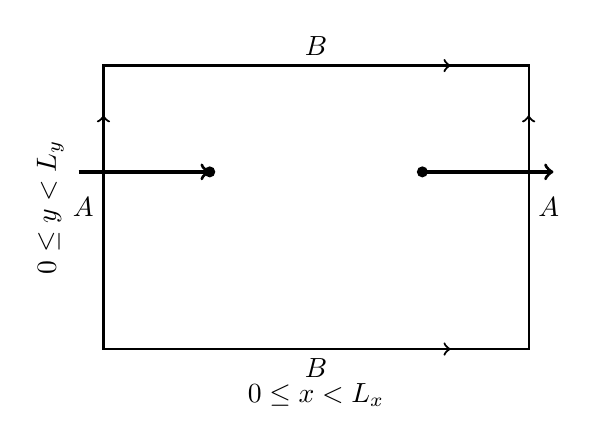
\begin{tikzpicture}[x=0.9cm,y=0.9cm]
\draw[thick] (0,0) rectangle (6,4);
\draw[->,thick] (0,0.7) -- (0,3.3);
\draw[->,thick] (6,0.7) -- (6,3.3);
\draw[->,thick] (1.1,0) -- (4.9,0);
\draw[->,thick] (1.1,4) -- (4.9,4);
\node[left] at (0,2) {$A$};
\node[right] at (6,2) {$A$};
\node[below] at (3,0) {$B$};
\node[above] at (3,4) {$B$};
\draw[->,very thick] (4.5,2.5) -- (6.35,2.5);
\draw[->,very thick] (-0.35,2.5) -- (1.5,2.5);
\fill (4.5,2.5) circle (2pt);
\fill (1.5,2.5) circle (2pt);
\node at (3,-0.65) {$0\leq x<L_x$};
\node[rotate=90] at (-0.75,2) {$0\leq y<L_y$};
\end{tikzpicture}
\caption{Một không gian tuần hoàn hai chiều: các cạnh mang cùng nhãn được đồng nhất, nên một hạt đi qua một cạnh sẽ xuất hiện lại ở điểm tương ứng trên cạnh đối diện.}
\end{figure}

\begin{classroomqa}
\lecturetimestamp{01:50:58}
\audiencequestion{Cấu trúc tuần hoàn biểu diễn không gian, hay các vật trong không gian?}
\lecturerresponse{Nó biểu diễn không gian. Các vật và các trường sống trong không gian đó và tuân theo các phép đồng nhất của nó. Tính tuần hoàn được áp đặt để kiểm soát bài toán thể tích vô hạn; nó được loại bỏ bằng cách lấy thể tích lớn và thay các tổng theo xung lượng bằng các tích phân.}
\end{classroomqa}

Tương tự ba chiều là một hình lập phương với ba cặp mặt đối diện được đồng nhất. Mặt trái và mặt phải là cùng một mặt, mặt trên và mặt dưới là cùng một mặt, và mặt trước và mặt sau là cùng một mặt. Một hạt đi qua bất kỳ mặt nào cũng xuất hiện lại qua mặt đối ứng đã được đồng nhất với nó.\footnote{Hình lập phương tuần hoàn và ba cặp mặt được đồng nhất của nó được trình bày từ 01:51:27--01:52:17. Phương trình được hiển thị cho \(k_i\) là cách viết lại theo từng thành phần của điều kiện trước đó \(kL=2\pi n\), áp dụng cho ba hướng tuần hoàn.} Ba thành phần xung lượng tuân theo
\begin{equation}
k_i=\frac{2\pi n_i}{L_i},
\qquad i=x,y,z,
\end{equation}
với một số nguyên \(n_i\) cho mỗi hướng. Các xuyến có thể được định nghĩa trong bất kỳ số chiều nào theo cùng quy tắc ấy.

\begin{figure}[t]
\centering
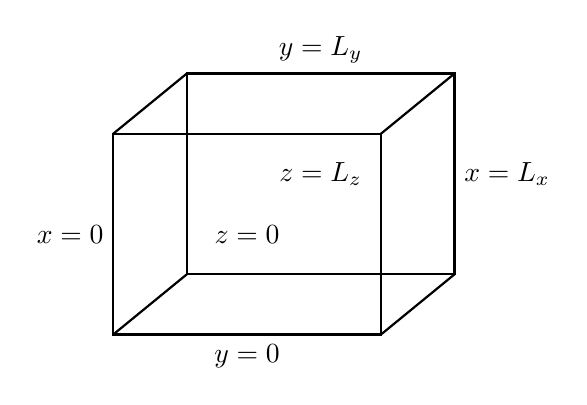
\begin{tikzpicture}[scale=0.85]
\draw[thick] (0,0) rectangle (4,3);
\draw[thick] (1.1,0.9) rectangle (5.1,3.9);
\draw[thick] (0,0) -- (1.1,0.9);
\draw[thick] (4,0) -- (5.1,0.9);
\draw[thick] (4,3) -- (5.1,3.9);
\draw[thick] (0,3) -- (1.1,3.9);
\node[left] at (0,1.5) {$x=0$};
\node[right] at (5.1,2.4) {$x=L_x$};
\node[below] at (2,0) {$y=0$};
\node[above] at (3.1,3.9) {$y=L_y$};
\node at (2,1.5) {$z=0$};
\node at (3.1,2.4) {$z=L_z$};
\end{tikzpicture}
\caption{Một không gian tuần hoàn ba chiều dưới dạng một hình lập phương trong đó mỗi cặp mặt đối diện được đồng nhất.}
\end{figure}

\begin{classroomqa}
\lecturetimestamp{01:52:20}
\audiencequestion{Lý thuyết trường có chọn một kích thước lưới vật lý cho không gian không?}
\lecturerresponse{Đó là một câu hỏi có tính suy đoán. Với các mục đích thực hành ở đây, không gian là liên tục. Các lượng tử là hạt, không phải các ô của một lưới không gian. Trong cấu trúc đường tròn, cái trở nên rời rạc là xung lượng; vị trí vẫn liên tục và tuần hoàn.}
\end{classroomqa}

\editorialnote{Một đoạn dài bị hư hỏng trong phần trao đổi về kích thước lưới có nhắc đến các thang Planck, nhưng không bảo toàn được một khẳng định nào có thể phục dựng về tính rời rạc cơ bản của không gian. Ở đây không suy ra một khẳng định như vậy.}

Tính rời rạc của \(k\) hoàn toàn xuất phát từ việc áp đặt một hàm sóng tuần hoàn. Điều đó không phải là bằng chứng rằng bản thân tọa độ \(x\) nằm trên một mạng. Việc đặt câu hỏi liệu không gian có thể có một cấu trúc vi mô cơ bản hay không là chính đáng, nhưng đó là một vấn đề riêng biệt, mang tính suy đoán.

\section{Fermion và các trường ngoài}

Các mode boson cho phép mọi số chiếm đóng không âm. Fermion đòi hỏi hành vi ngược lại: nguyên lý loại trừ Pauli cấm hai fermion đồng nhất chiếm cùng một trạng thái.

\begin{classroomqa}
\lecturetimestamp{01:55:13}
\audiencequestion{Việc thay các giao hoán tử bằng các phản giao hoán tử có cho ta lý thuyết fermion đơn giản nhất không?}
\lecturerresponse{Về cơ bản là có. Giao hoán tử là \([A,B]=AB-BA\), còn phản giao hoán tử là \(\{A,B\}=AB+BA\). Đại số tạo-hủy fermion tương ứng thực thi nguyên lý loại trừ Pauli: không thể đặt thêm một fermion đồng nhất thứ hai vào một trạng thái đã bị chiếm. Phần lý thuyết chi tiết được hoãn lại.}
\end{classroomqa}

Hai tích này khác nhau bởi một dấu:
\begin{equation}
[A,B]=AB-BA,
\qquad
\{A,B\}=AB+BA.
\end{equation}
Giao hoán tử là phản đối xứng dưới phép hoán đổi, còn phản giao hoán tử thì đối xứng. Nếu một phản giao hoán tử bằng không, thì
\begin{equation}
\{A,B\}=0
\quad\Longrightarrow\quad
AB=-BA.
\end{equation}
Đối với một cặp như vậy, việc hoán đổi hai toán tử fermion làm đổi dấu. Điều này khác thường hơn phép giao hoán thông thường, nơi \([A,B]=0\) cho \(AB=BA\). Việc thay các giao hoán tử boson bằng đại số phản giao hoán tương ứng là thay đổi toán học dẫn đến fermion; phần triển khai chi tiết của nó được hoãn lại.

Phản giao hoán đảo ngược hành vi thống kê thấy ở boson. Không có sự dồn tích được kích thích của các fermion đồng nhất trong một mode; việc mode đó đã bị chiếm sẽ ngăn một fermion đồng nhất khác đi vào nó. Vì một trạng thái fermion đơn lẻ nhiều nhất chỉ có thể chứa một fermion đồng nhất, nên không thể thu được giới hạn trường cổ điển bằng cách đặt một số lượng tùy ý lớn các hạt ấy vào chính trạng thái đó.

\begin{classroomqa}
\lecturetimestamp{01:58:03}
\audiencequestion{Làm sao một hạt alpha có thể là boson nếu nó được tạo thành từ các fermion?}
\lecturerresponse{Một hệ hợp thành liên kết chứa một số chẵn thành phần fermion có thể có thống kê boson. Việc đặt nhiều boson hợp thành như vậy vào cùng một trạng thái tổng thể không đồng nghĩa với việc đặt các thành phần fermion riêng lẻ của chúng vào một trạng thái một-hạt đồng nhất duy nhất.}
\end{classroomqa}

Thống kê của hệ hợp thành liên quan đến vật liên kết như một toàn thể. Vì thế, các thành phần fermion có thể kết hợp thành một đối tượng cư xử như một boson mà không vi phạm nguyên lý loại trừ đối với chính các thành phần đó.

\begin{classroomqa}
\lecturetimestamp{01:58:33}
\audiencequestion{Các trường ngoài được đưa vào như thế nào?}
\lecturerresponse{Cho tới nay, chưa có trường nền ngoài nào được đưa vào trong phép xây dựng này. Một trường như vậy có thể được cho trước như một trường cổ điển, hoặc được biểu diễn bằng cơ học lượng tử bởi một trạng thái chứa một số lượng lớn lượng tử.}
\end{classroomqa}

Để hai cách mô tả phù hợp với nhau, trạng thái có số chiếm đóng lớn phải được chuẩn bị thích hợp và có tính kết hợp pha; chỉ riêng số hạt là không đủ.\footnote{Phần trao đổi trên cung cấp thang nhiều-lượng-tử. Ở đây, tính kết hợp pha được nêu ra như điều kiện bổ sung ngăn không cho chỉ riêng số chiếm đóng lớn bị ngộ nhận là một trường cổ điển.} Trong miền bán cổ điển đó, tác dụng của chúng trùng khớp với nhau, sai khác chỉ bởi những độ lệch lượng tử nhỏ. Đây là một điều kiện nhất quán cơ bản. Trường điện từ phải mô tả các photon rời rạc khi từng lượng tử riêng lẻ trở nên quan trọng, nhưng một trạng thái có tính kết hợp pha thích hợp, chứa nhiều photon, cũng phải tái hiện được tác dụng quen thuộc của một sóng điện từ cổ điển.
